
\begin{figure}[H]
		\centering
		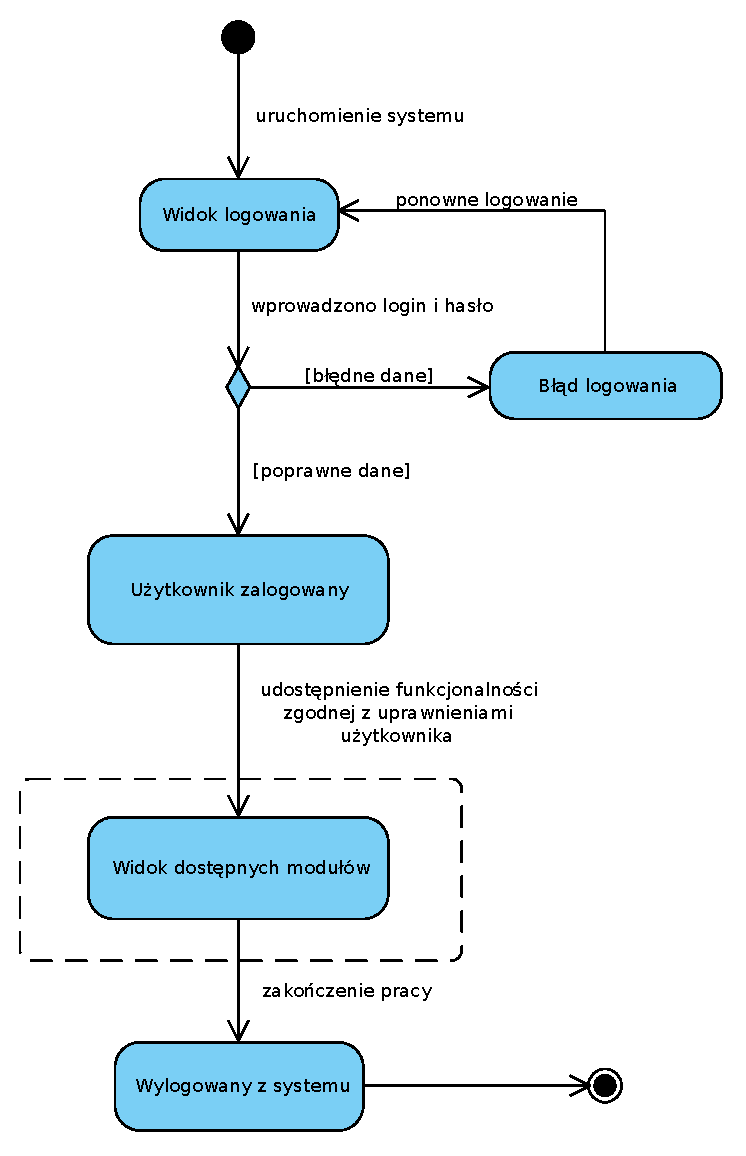
\includegraphics[width=.8\textwidth]{img/AD/STDmain.eps}
		\caption{Ogólny diagram STD}
\end{figure}

Na powyższym diagramie widzimy ogólny zarys zachowania systemu, poniżej pokażemy jego zachowanie w zależności od tego jaki użytkownik z niego korzysta, czyli pokażemy interpretacje "widoku poszczególnych modułów" dla użytkowników.

\subsection{Obsługa klienta}
\begin{landscape}
		\begin{figure}[H]
			\centering
			\centerline{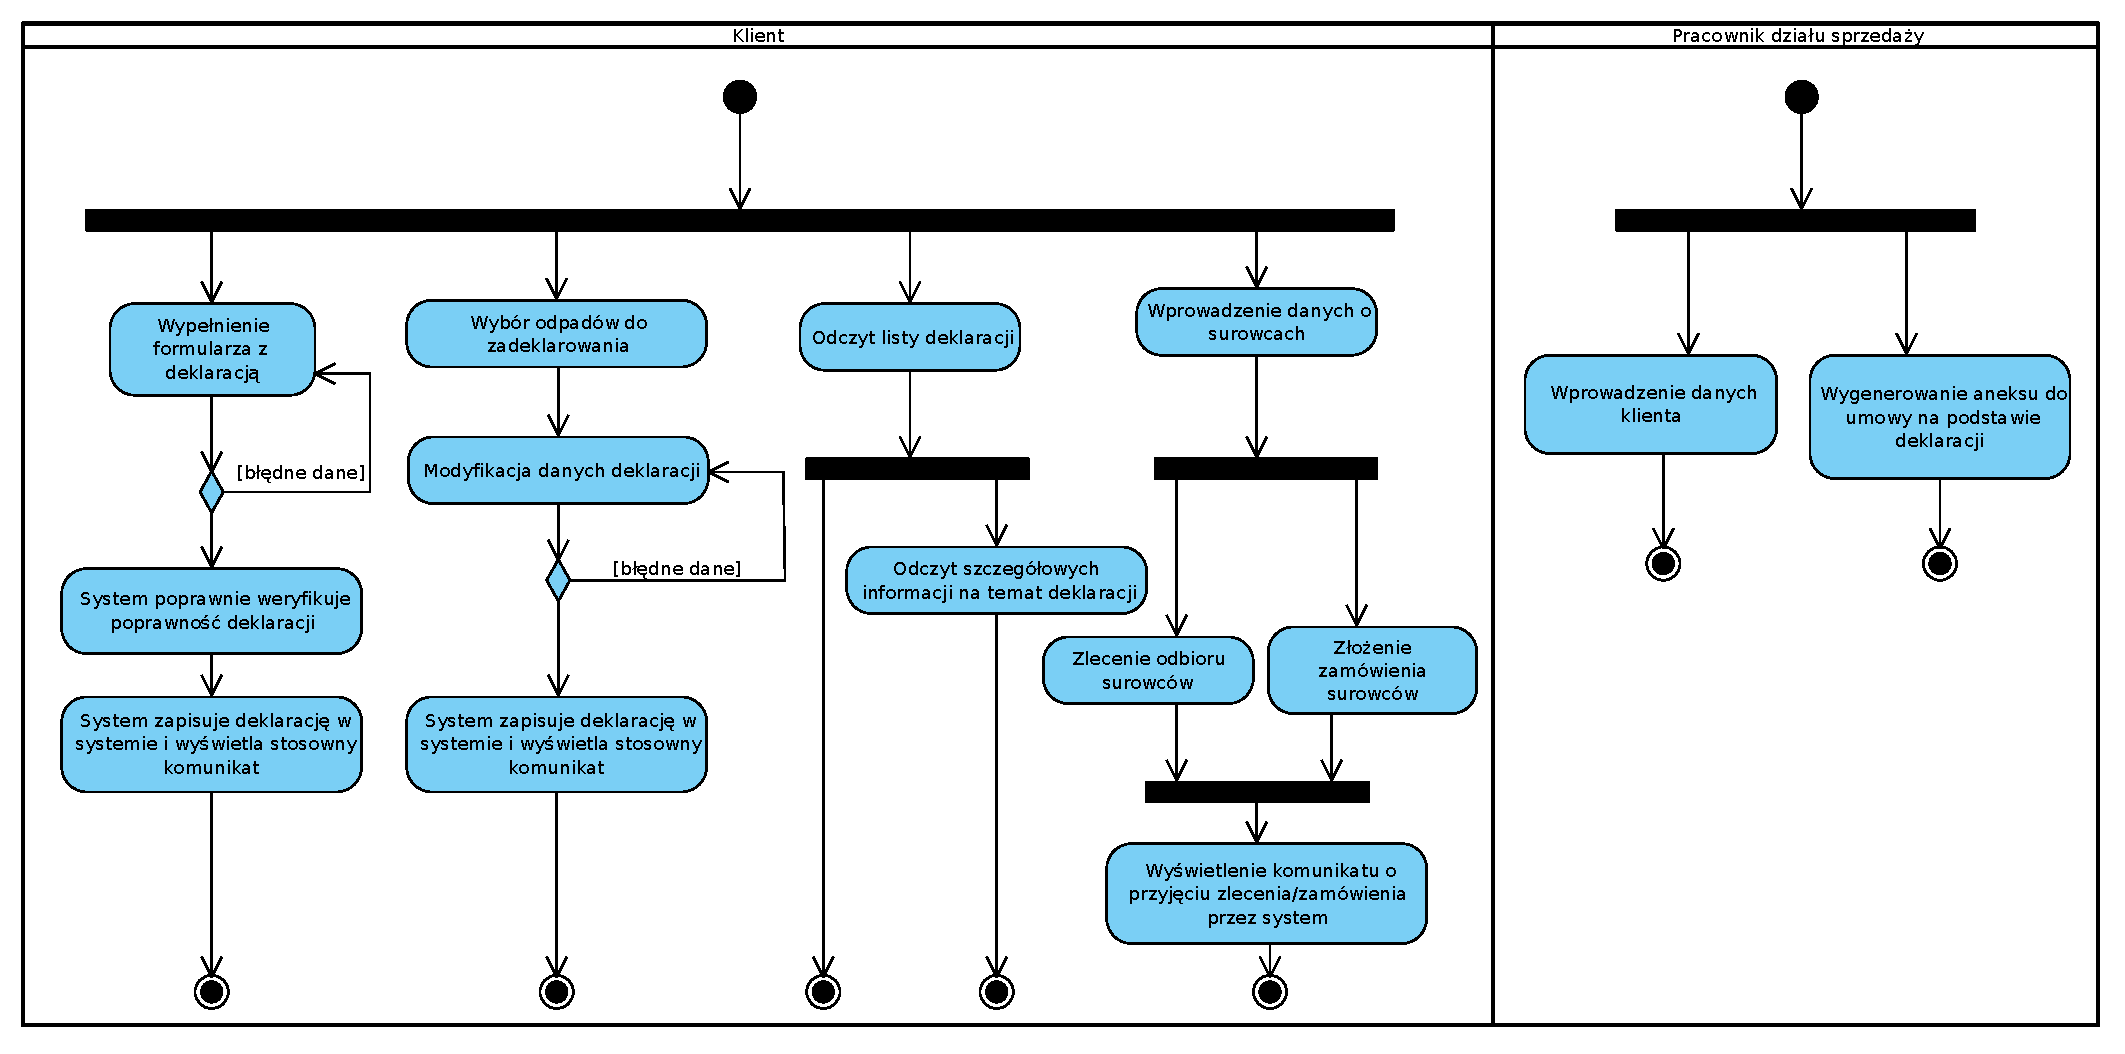
\includegraphics[width=24cm]{img/AD/klient.eps}}
		\caption{Diagram aktywności dla obsługi klienta}
		\end{figure}
\end{landscape}

\subsection{Obsługa skupu}
	\begin{figure}[H]
		\centering
		\centerline{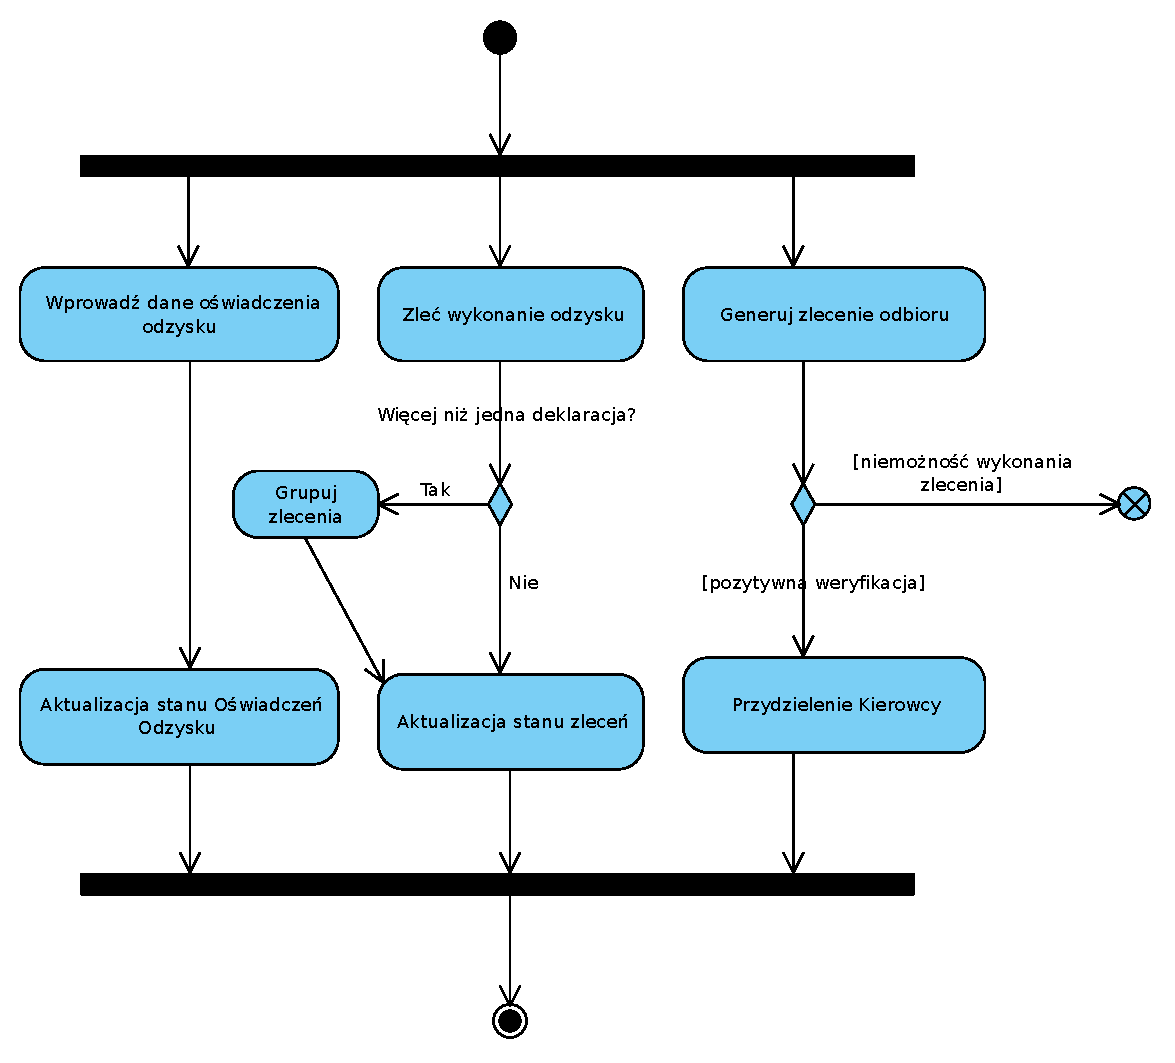
\includegraphics[width=1.2\textwidth]{img/AD/skup.eps}}
		\caption{Diagram aktywności dla obsługi skupu}
	\end{figure}

\subsection{Obsługa księgowości}
	\begin{figure}[H]
		\centering
		\centerline{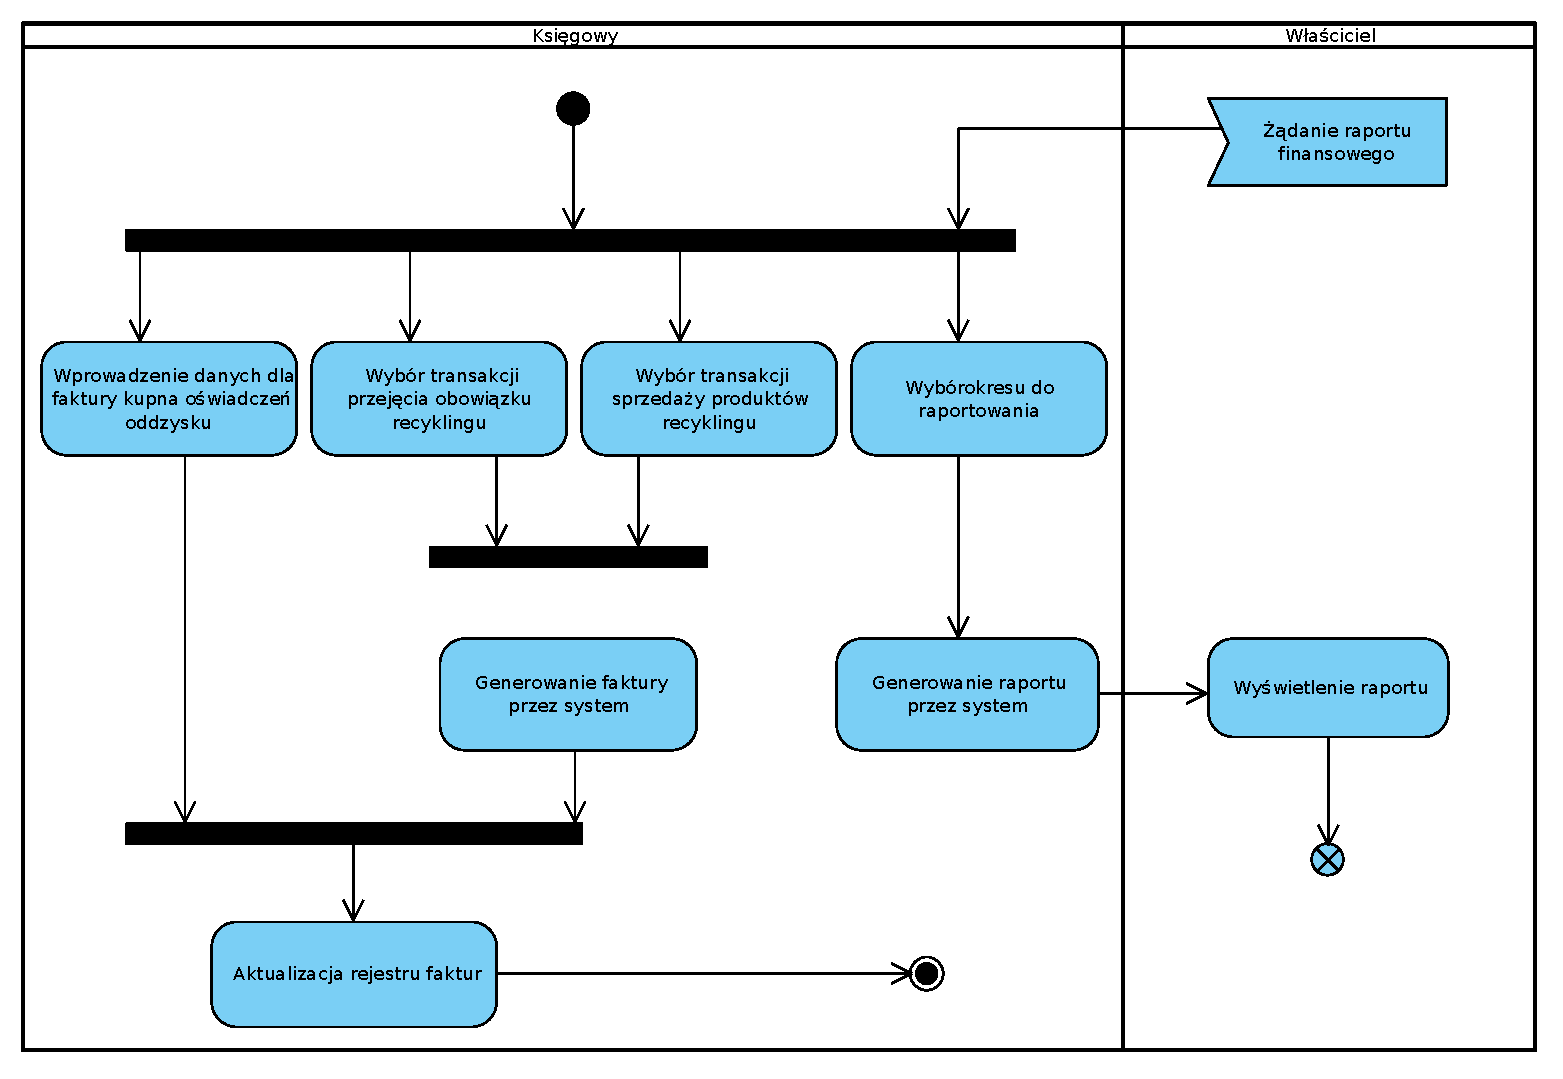
\includegraphics[width=1.2\textwidth]{img/AD/ksiegowosc.eps}}
		\caption{Diagram aktywności dla obsługi księgowości}
	\end{figure}

\subsection{Obsługa magazynu}
	\begin{figure}[H]
		\centering
		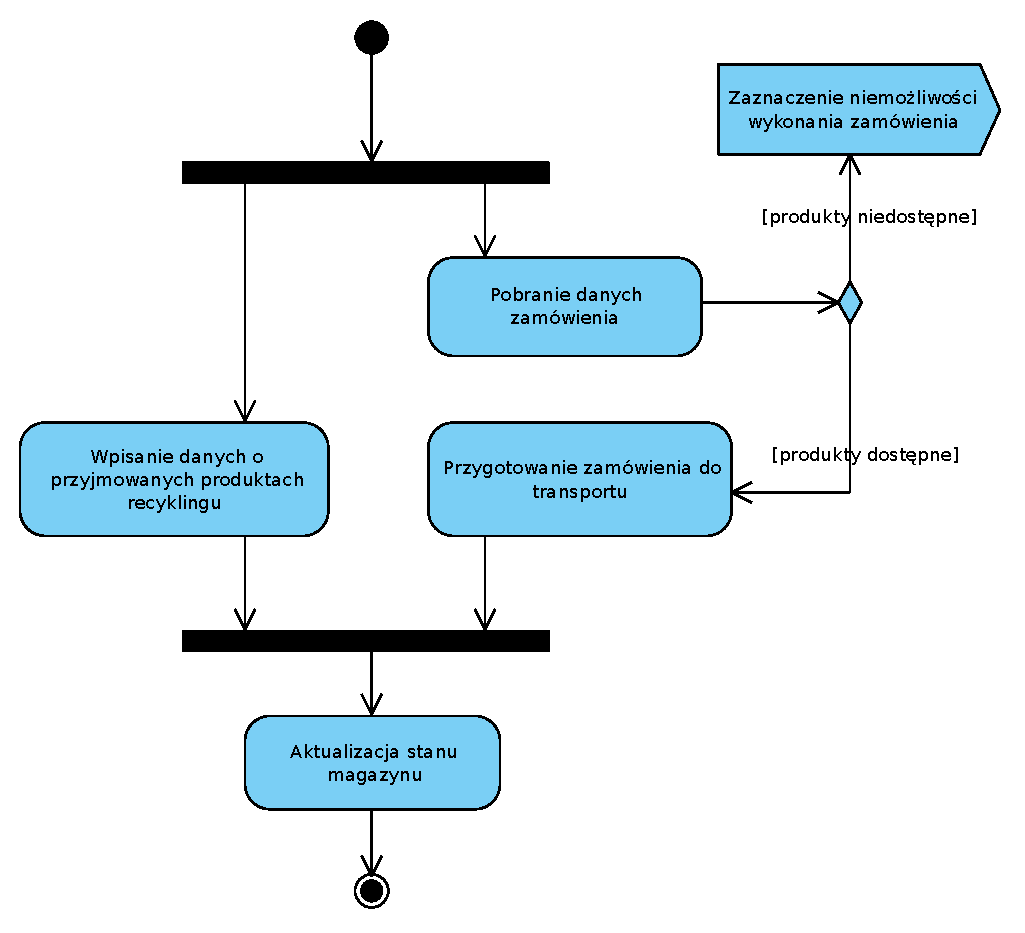
\includegraphics[width=.9\textwidth]{img/AD/magazyn.eps}
		\caption{Diagram aktywności dla obsługi magazynu}
	\end{figure}

\subsection{Obsługa kierowców}
	\begin{figure}[H]
		\centering
		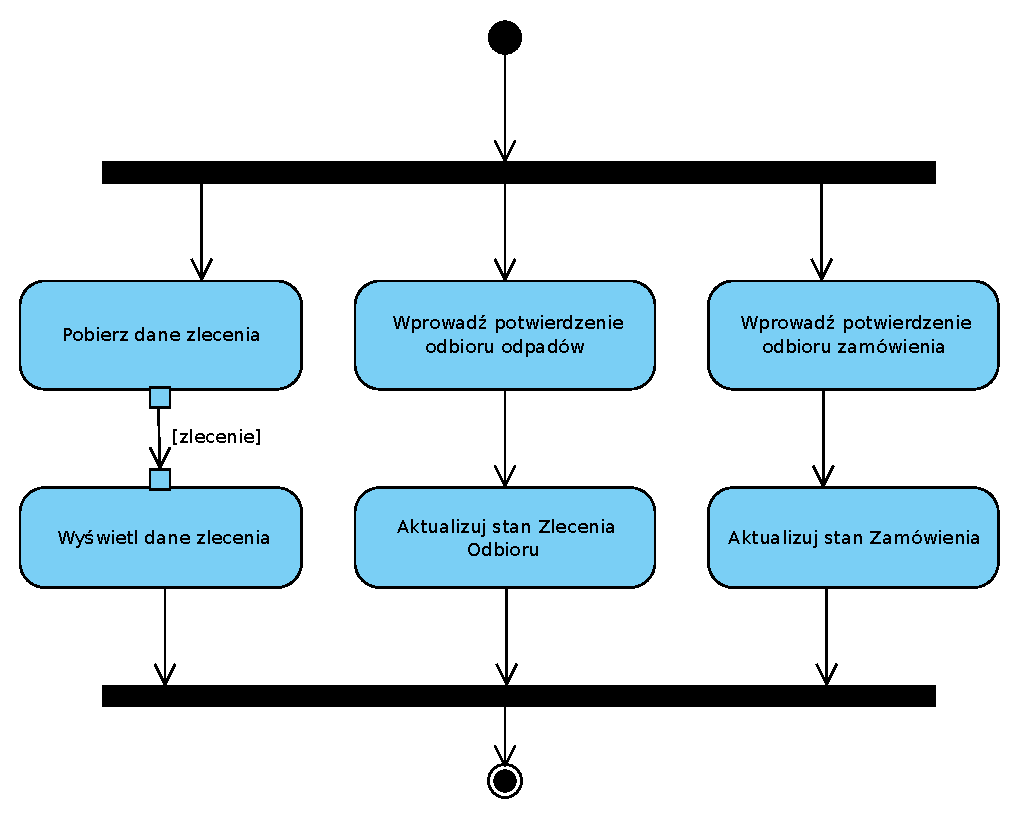
\includegraphics[width=.9\textwidth]{img/AD/kierowca.eps}
		\caption{Diagram aktywności dla obsługi kierowców}
	\end{figure}